\chapter{绪论}\label{chap:introduction}

本章节主要介绍本文工作的研究背景和意义。首先,本文对一些基本概念给出定义,包括SMT问题、非线性实数理论(NRA)、解空间以及符号一致胞腔。本文还会介绍目前的几种主流求解算法以及局限性,引出本文工作的研究动机。接着,本文会针对工作的几个创新点展开,详细阐述算法的设计。最后,本文将总结论文的整体结构。

\section{研究背景及意义}
随着信息技术的发展,软硬件系统的正确性和安全性日益成为人们关注的话题。现有的一些验证技术使用诸如模型检查、定理证明等手段将问题转化成为可满足性模理论(Satisfiability Modulo Theories, SMT)问题,并通过求解器求解。因此,SMT求解算法的设计对工业生产、科学研究等领域具有重要意义。针对特定的约束类型,如何设计高效的求解算法,在短时间内求解更多的样例成为SMT研究的一个重点。基于此,研究一种高效求解SMT问题的算法具有很高的理论意义与实际价值。

\subsection{可满足性模理论问题(SMT Problem)}
% 介绍SMT问题
可满足性模理论问题(SMT)是一种在计算机科学中常见的问题类型,它组合了布尔可满足性问题(SAT)和一些理论约束。每一个约束一般可以表示为对变量集合取值范围的限制,当一组变量的赋值满足了所有约束时,当前赋值被称为SMT问题的一组解。SMT求解可以理解为寻找一组解或者证明不存在解的过程。SMT问题的一个挑战在于囊括理论的复杂性,比如算术理论、位向量理论等,不同理论需要的求解策略也不同。除此之外,SMT问题涉及到的变量个数与约束个数十分庞大,解空间规模基本上呈指数关系,这也就造成了目前的求解器很难在短时间内处理十分庞大的SMT问题。

% SMT的应用
SMT问题在很多领域有广泛应用,常用于符号执行\cite{KLEE, DART},程序验证\cite{AnalysisSymbol,VerificationSMT},程序生成\cite{synthesis1},自动机学习\cite{Automata1,automata2}以及神经网络验证等\cite{NN1,NN2,NN3,NN4}。非线性实数理论一般广泛应用于信息物理系统\cite{CPS1,CPS2,CPS3},程序终止条件的秩函数生成\cite{LeikeH15,HeizmannHLP13},非线性混成自动机的分析\cite{CimattiMT12}等。一般来说,这些问题会把需要验证的条件编码成为SMT问题,然后交给后端的求解器取处理。比如,在符号执行中约束包括程序的分支条件,需要对程序可能执行的每一条路径进行搜索,从而确保最终程序的状态符号认为的要求,这些条件最终被编码成为SMT问题中的约束,整个问题转化为全部约束是否可以同时满足,即SMT问题。

% SMT的求解
目前关于SMT求解的研究基本可以分为完备搜索算法和启发式搜索算法。完备搜索算法主要的思想是通过搜索SMT问题的一部分空间,然后在遇到冲突的情况下通过推理和回溯完成对当前冲突区域的剪枝,以避免后续搜索遇到相同冲突,算法在所有变量得到赋值后结束。一般来说,完备算法因为其很强的推理能力成为主流算法,但整体推理的时间和空间复杂度较高,面对大规模的样例容易消耗过多的计算资源。启发式方法一般借助一些人工的启发式优化策略,比如引入随机等,来更好地完成整个搜索过程。启发式方法一般会针对特殊的约束类型采取不同的启发式策略,因此其求解效果可能会根据样例的形式不同而产生不同的效果。在处理大规模样例中,启发式效果对计算资源的消耗较少,有时会得到比完备算法更好的结果。本文接下来会重点概述几种不同算法的求解思路。

% SMT的完备算法
完备算法一般也成为系统搜索算法,可以同时处理约束可满足以及不可满足的情况。SMT的完备算法一般包括CDCL(T)\cite{NieuwenhuisOT06}和MCSAT算法\cite{JovanovicM12,MouraJ13},其共同的思路是不断尝试新的赋值,在遇到冲突时通过冲突分析学习新的子句,通过不断试错缩小需要探索的解空间,直到最终找到满足所有约束的一组解,或者排除整个解空间从而证明原公式不可被满足。非线性实数理论一般需要通过柱形代数分解(CAD)\cite{Caviness2004QuantifierEA}进行量词消去,从而学习到特定冲突下的新子句。这方面的研究包括应用CAD的变种\cite{AbrahamDEK21},对CAD投影设计启发式的变量顺序\cite{LiXZZ23}等。
除了上述两种算法之外,近年来一些其他算法也在SMT求解上取得了不错的效果,包括增量线性化\cite{Incremental2},区间约束传播\cite{KhanhO12,TungKO17}和亚热带方法\cite{FontaineOSV17,NalbachA23}。这些方法一般作为求解器插件使用,可以在特定的样例进行快速处理。

% SMT的优化方法
近年来,一些基于优化方法常用来检测给定区域内是否存在符合多项式组的解,进而应用到了SMT问题上。其中,Cimatti等人的工作\cite{CimattiGLS22}首次应用全局优化的方法去寻找初始解,然后通过迭代寻找附近的可行解。Ni等人的工作也使用了优化方法去寻找可行解\cite{NiWX23},然后通过解方程\cite{LiXZ23b}等手段求出一个精确解。

% dReal求解器
Gao等人引入$\delta$-完备($\delta-complete$)决策程序的概念,并基于此设计了解决非线性约束的dReal求解器。与一般SMT求解器不同的是,dReal支持对指数函数和三角函数的求解。其中$\delta$-完备包括$\delta$-满足($\delta-sat$)和不可满足(unsat),通过松弛输入的公式来解决更宽泛问题的效果。本文的工作主要借鉴了这种松弛的想法来加速局部搜索的迭代。和dReal求解器不同的是,我们的算法最终仍然会返回一个严格满足所有约束的精确解。

% SMT局部搜索方法
局部搜索算法是本文工作的重点,也是近年来求解可满足样例的重点。局部搜索算法一般从一个完全赋值开始,针对当前尚且不可满足的约束设计操作,使用评价函数筛选合适的操作进行迭代,最终通过不断在邻域中搜索输出满足所有约束的一组赋值。其主要优点是对特定样例的求解效果很好,并且能够在很短的时间内找到足够好的一组解。主要缺点包括容易陷入局部最优、操作的设计和评价函数的设计较为困难等。局部搜索一般不可用于求解不可满足的样例。目前主流的局部搜索算法支持线性整数逻辑\cite{CaiLZ22}、非线性整数逻辑\cite{CaiLZ2023}、多线性样例\cite{multilinear}和部分多项式理论\cite{LiXZ23}。本文提出了第一个可以覆盖全部非线性实数理论的局部搜索算法。

% 主要工作概述
\section{论文主要工作}
本文重点关注非线性实数的SMT问题。本文主要讨论非线性实数问题求解的难点,并针对这些难点设计出合适的局部搜索算法,从而达到高效求解的效果。目前算法的主要难点是求解高次多项式约束需要太多求解时间,这些样例成为我们设计局部搜索算法的重点。

本工作主要在SMT-LIB\cite{BarFT-SMTLIB}上进行试验,在可满足样例上超越了目前的主流搜索算法。算法的创新性上,本文主要考虑以下几个方面:
\begin{itemize}
    \item 考虑通过设计更好地数据结构和迭代策略,针对实数问题的操作采样进行优化,以期望可以加速整体搜索过程;
    \item 针对非线性实数特有的无理数赋值问题,如何减少多项式计算上的时间消耗;
    \item 考虑非线性问题单变量无操作的情况,如何避免搜索陷入停滞的情况;
\end{itemize}

本文的局部搜索算法\textbf{LS\_NRA}整体流程如图\ref{fig:total}所示。本工作主要包括以下几个贡献:
\begin{itemize}
    \item 首先,本文通过分析非线性实数的解空间引入边界(boundary)数据结构,从而实现了可行域-分数对变量的缓存机制。本文还给出了邻居变量的定义以及边界的更新算法,从而可以保证算法的正确性以及数据结构的可复用性;
    \item 针对无理数赋值问题,本文借鉴dReal的做法,在强迫无理数赋值时引入等式松弛(relaxation)的概念,允许暂时的有理数赋值。在找到松弛解之后,本文给出了求解精确解的算法,保证了算法的正确性;
    \item 针对非线性问题独有的无单变量移动问题,本文给出了一个简单的迭代算法和前瞻策略(look-ahead),基本避免了算法停滞的现象;
    \item 本文增加了重启策略和预处理模块,相关工具在SMT-LIb上效果良好,可以在短时间内快速找到高次多项式的可满足赋值,打破了以往主流求解器的高次问题上的零求解。
\end{itemize}

\begin{figure*}[]
    \centering
    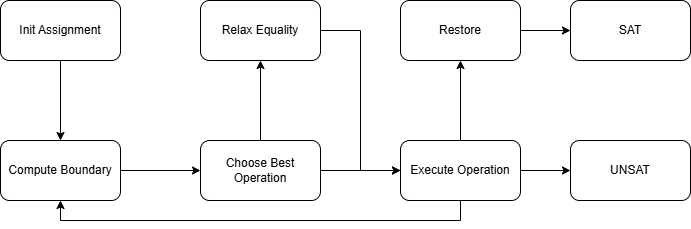
\includegraphics[width=0.9\columnwidth]{Img/LS_NRA.png}
    \bicaption {工具整体框架。} {Overall framework of LS\_NRA.}
    \label{fig:total}
\end{figure*}

\section{论文组织}
本文的后续章节按照以下方式组织:\\
第二章:介绍SMT问题的基本概念和解空间,并介绍目前主流的算法和研究现状。\\
第三章:介绍目前非线性实数理论的挑战和本文的设计思路及实现过程。\\
第四章:介绍预处理模块、重启策略和整体工具实现。\\
第五章:介绍实验设计和结果分析。\\
第六章:总结本文贡献,展望后续研究工作。